\chapter{Naprednije analize podataka}

	\section{Proučavanje međusobne ovisnosti atributa}
	
	\begin{figure}[H]
		\centering
		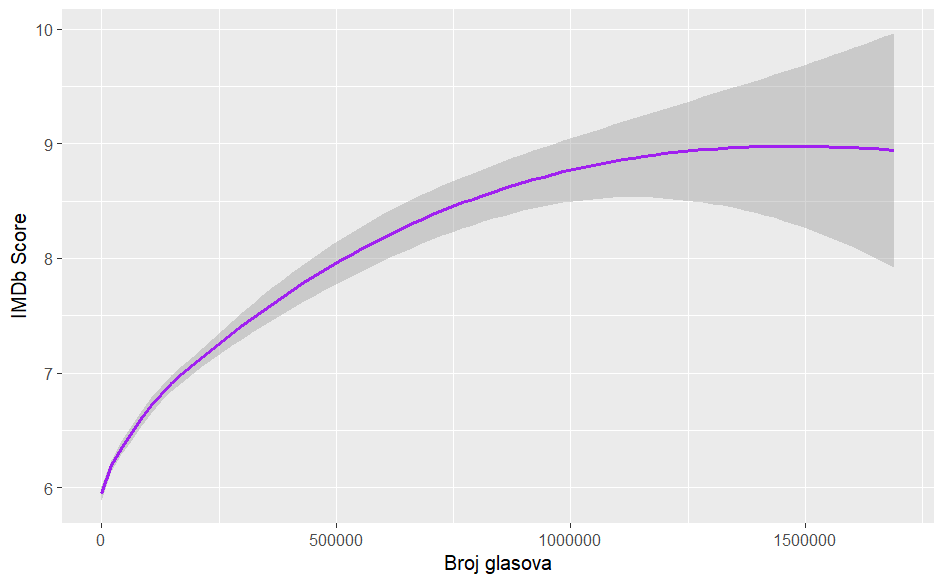
\includegraphics[width=15cm]{../figures/lucija_slozeni/glasoviocjena.png}
		\caption{IMDb ocjena u ovisnosti o broju glasova}
		\label{napredni1}
	\end{figure}
	
	\begin{figure}[H]
		\centering
		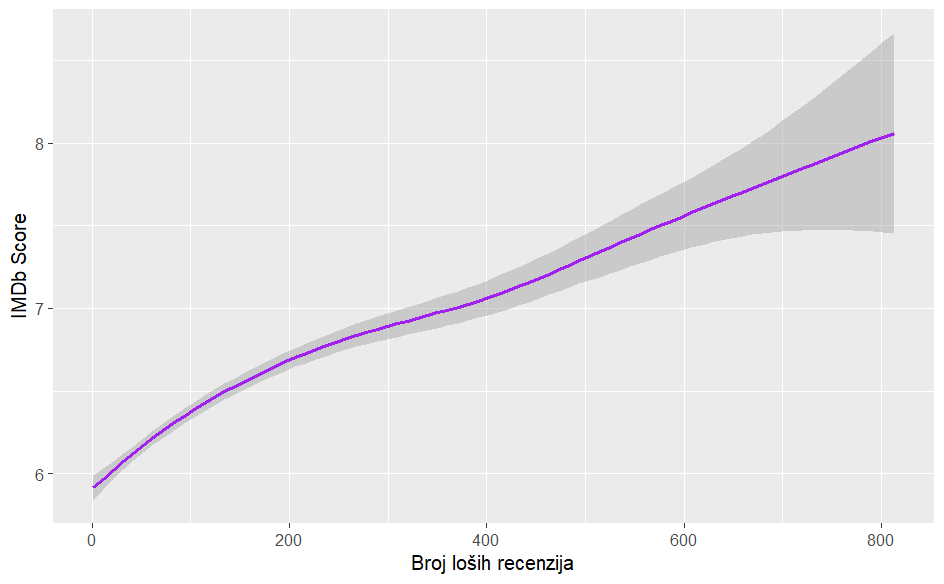
\includegraphics[width=15cm]{../figures/lucija_slozeni/loseocjena.png}
		\caption{IMDb ocjena u ovisnosti o broju loših recenzija}
		\label{napredni2}
	\end{figure}
	
	\begin{figure}[H]
		\centering
		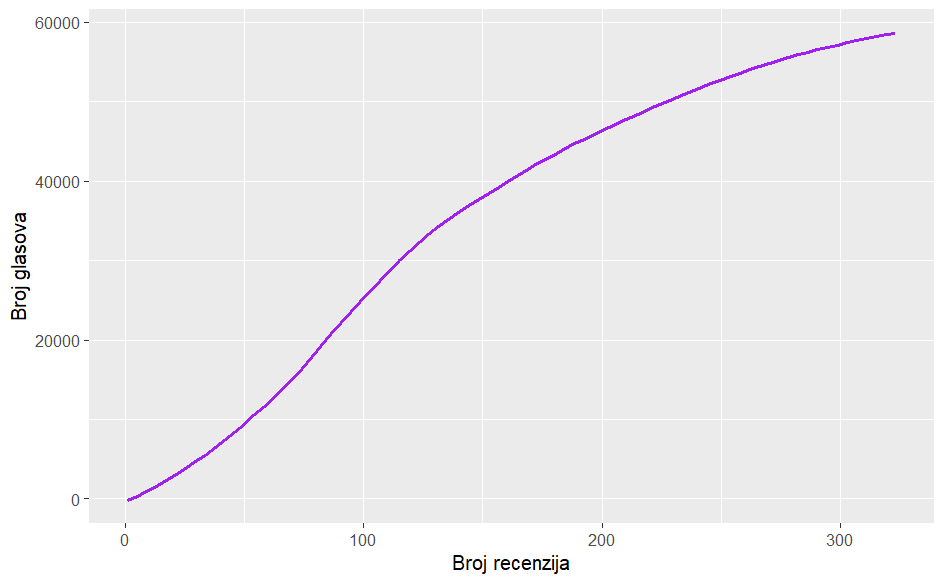
\includegraphics[width=15cm]{../figures/lucija_slozeni/recenzijeglasovi.png}
		\caption{Broj loših recenzija u ovisnosti o ukupnom broju recenzija}
		\label{napredni3}
	\end{figure}
	
	\begin{figure}[H]
		\centering
		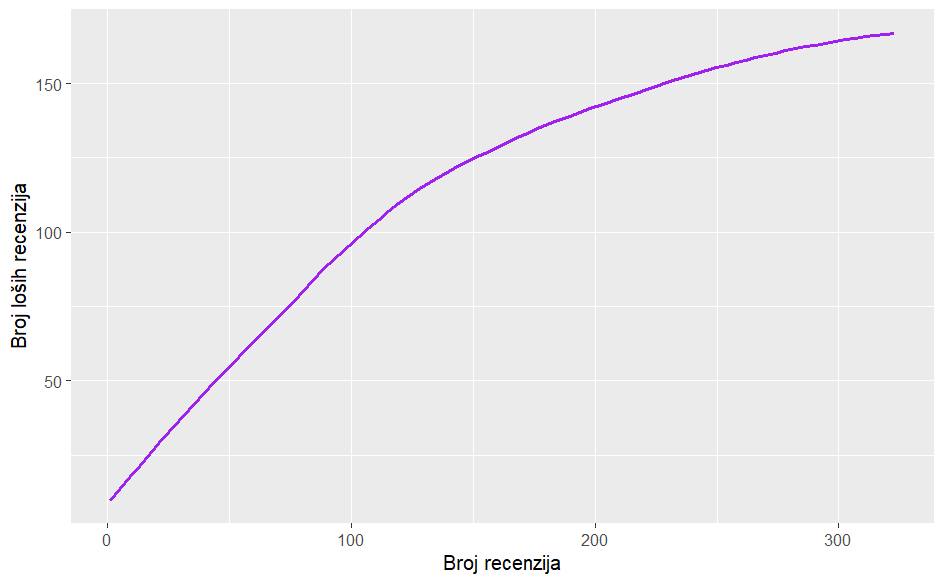
\includegraphics[width=15cm]{../figures/lucija_slozeni/recenzijelose.png}
		\caption{}
		\label{napredni4}
	\end{figure}
	
	\newpage
	
	\section{Dodatne zanimljive vizualizacije}
	
	Na slici \ref{filmovi_zanr} primjećujemo da je "Drama" najčešći žanr s najvećim ukupnim brojem filmova. Izdvajajući podatke o filmovima s tim žanrom, možemo prikazati popularnost žanra "Drama" po godinama. Iz vizualizacije na slici \ref{drama} dalo bi se zaključiti da popularnost \textit{eksplodira} u razdoblju od 1990. do 2016. godine, no to zapravo nije slučaj. Uzimajući u obzir ukupan broj filmova izdanih tih godina (vidi sliku \ref{filmovi_godine}), uviđamo da je veliki broj filmova s žanrom "Drama" zapravo rezultat općenitog povećanja produkcije filmova u tom razdoblju. Ako umjesto apsolutnog broja filmova promatramo udio filmova s žanrom "Drama"  u ukupnom broju filmova te godine, zaključujemo da je taj udio konstantan, prosječno 0.4805 (medijan 0.4976) za sve godine. 
	
	\begin{figure}[H]
		\centering
		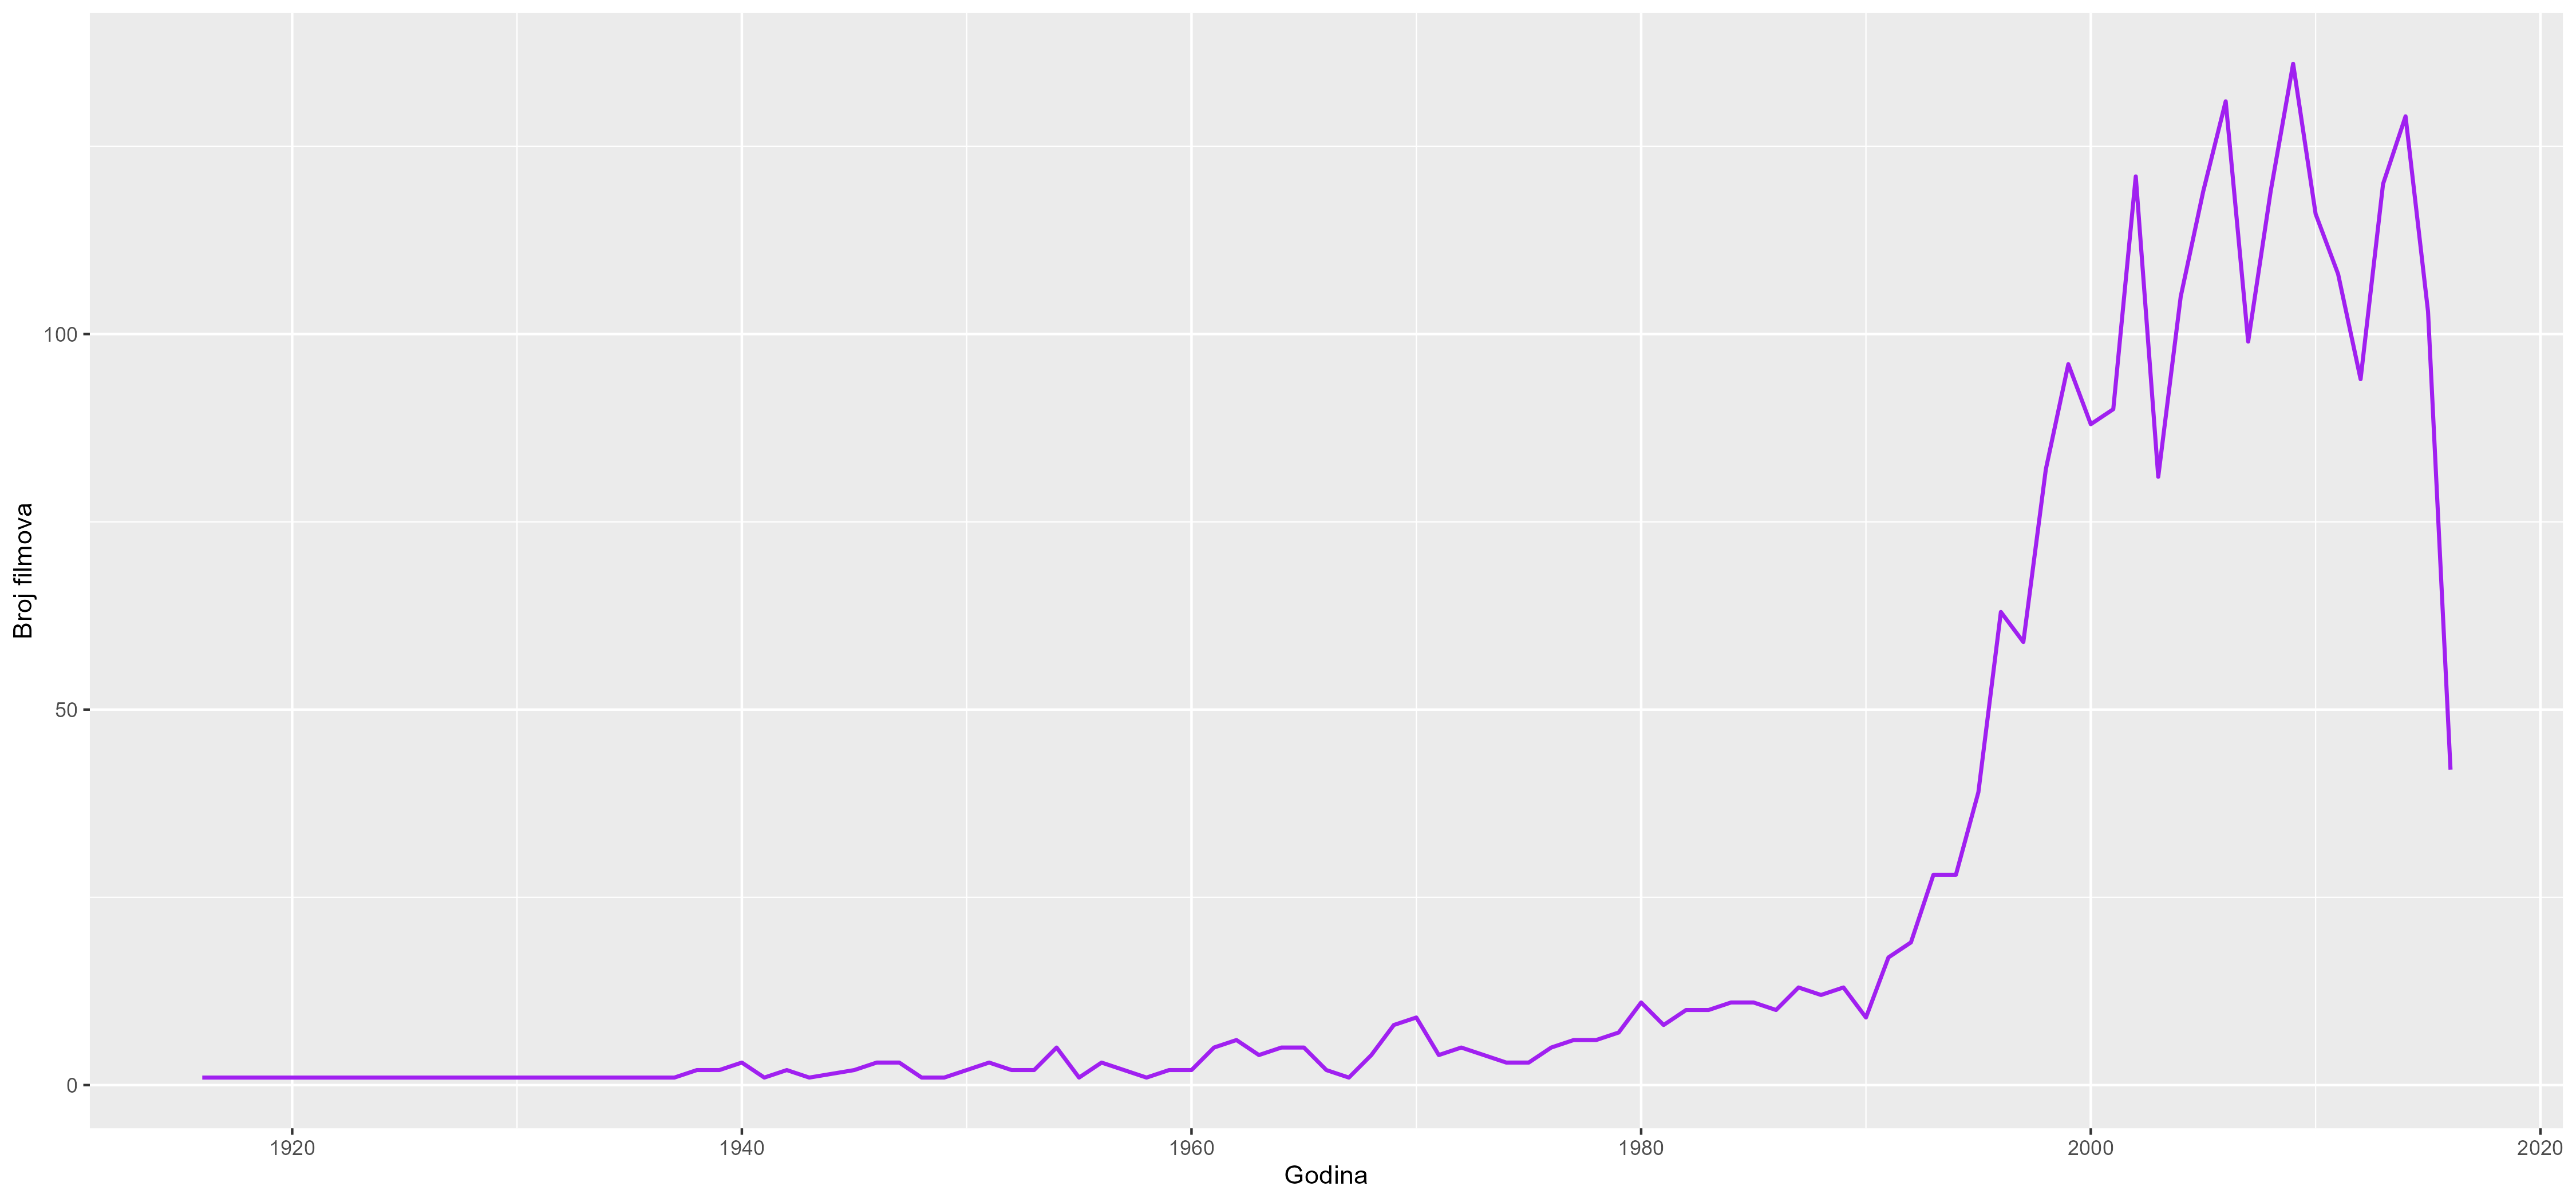
\includegraphics[width=15cm]{../figures/analysis/popularnost_drame.png}
		\caption{Broj filmova žanra "Drama" po godinama}
		\label{drama}
	\end{figure}
	
	Iz tablice \ref{redatelji_s_najvise_filmova} saznajemo da je Steven Spielberg redatelj koji je režirao najveći broj filmova iz ovog skupa podataka, njih ukupno 26. S ciljem uvida u trend IMDb ocjena filmova tog redatelja i usporedbe s novim podacima stvaramo graf na slici \ref{spielberg}. Ljubičaste točke na grafu predstavljaju godine premijere filmova redatelja Stevena Spielberga i njihove odgovarajuće IMDb ocjene. Tim je točkama dodana glatka krivulja (ljubičasta isprekidana linija) koja ilustrira trend ocjena tijekom godina dobivena korištenjem metode \texttt{geom\_smooth} i postavljanjem \texttt{method = 'loess'}. Dodatno, ružičastom su bojom prikazani podaci o  filmovima istog redatelja od 2017. do 2022. godine. Novim je podacima dodana i regresijska krivulja (metoda \texttt{geom\_smooth} i \texttt{method = 'lm'}). 
	
	\begin{figure}[H]
		\centering
		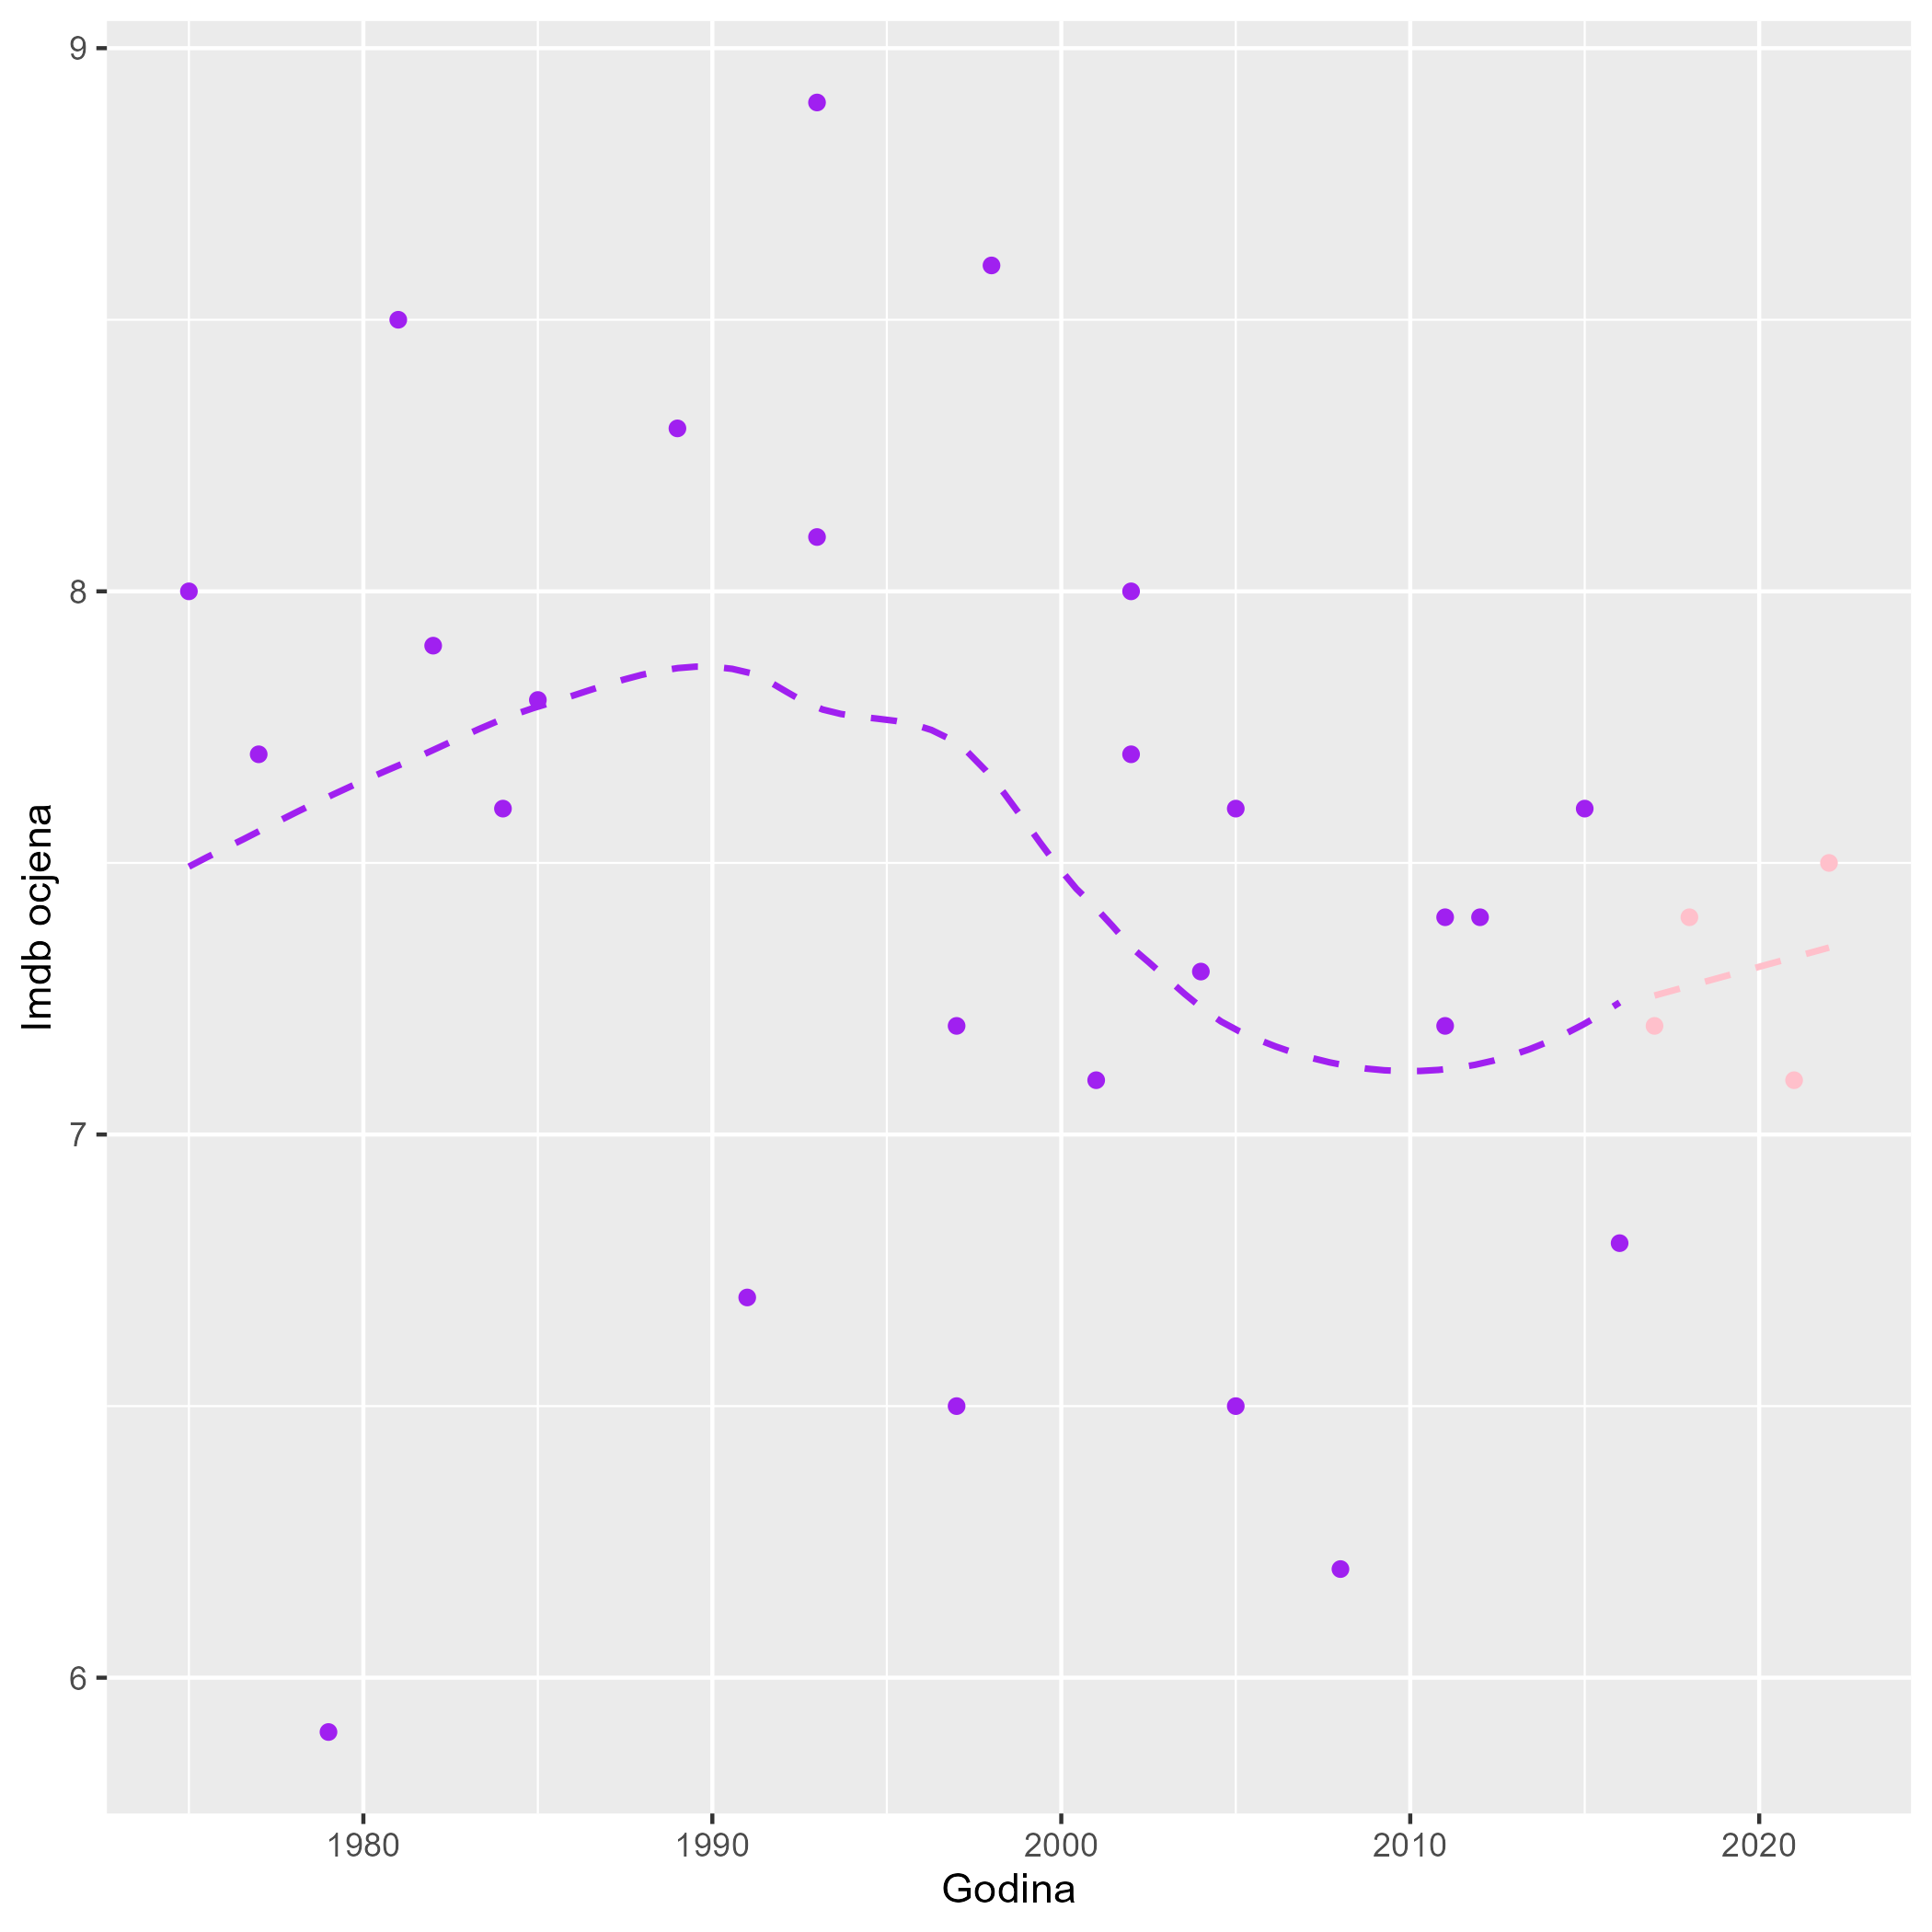
\includegraphics[width=15cm]{../figures/analysis/spielberg.png}
		\caption{IMDb ocjene filmova Stevena Spielberga po godinama}
		\label{spielberg}
	\end{figure}
	
	Drugi po redu stupac s najviše nedostajućih (\textit{NA}) vrijednosti stupac je \texttt{budget}. Taj stupac sadrži podatke o trošku proizvodnje (budžetu) filma u američkim dolarima. Prilagodbom iznosa navedenih u stupcu \texttt{budget} uzevši u obzir stope inflacije\footnote{https://www.minneapolisfed.org/about-us/monetary-policy/inflation-calculator/consumer-price-index-1913-} dobivamo ekvivalentne iznose za 2016. godinu (posljednja godina za koju imamo zapise o filmovima u ovom skupu podataka). Sada možemo uspoređivati prosječni iznos budžeta filmova po godinama. Graf na slici \ref{budzet} pokazuje značajne oscilacije prosječnog budžeta, s oštrim usponima i padovima, no lako je primijetiti rast minimalnog iznosa prosječnog budžeta kroz godine.
	  
	\begin{figure}[H]
		\centering
		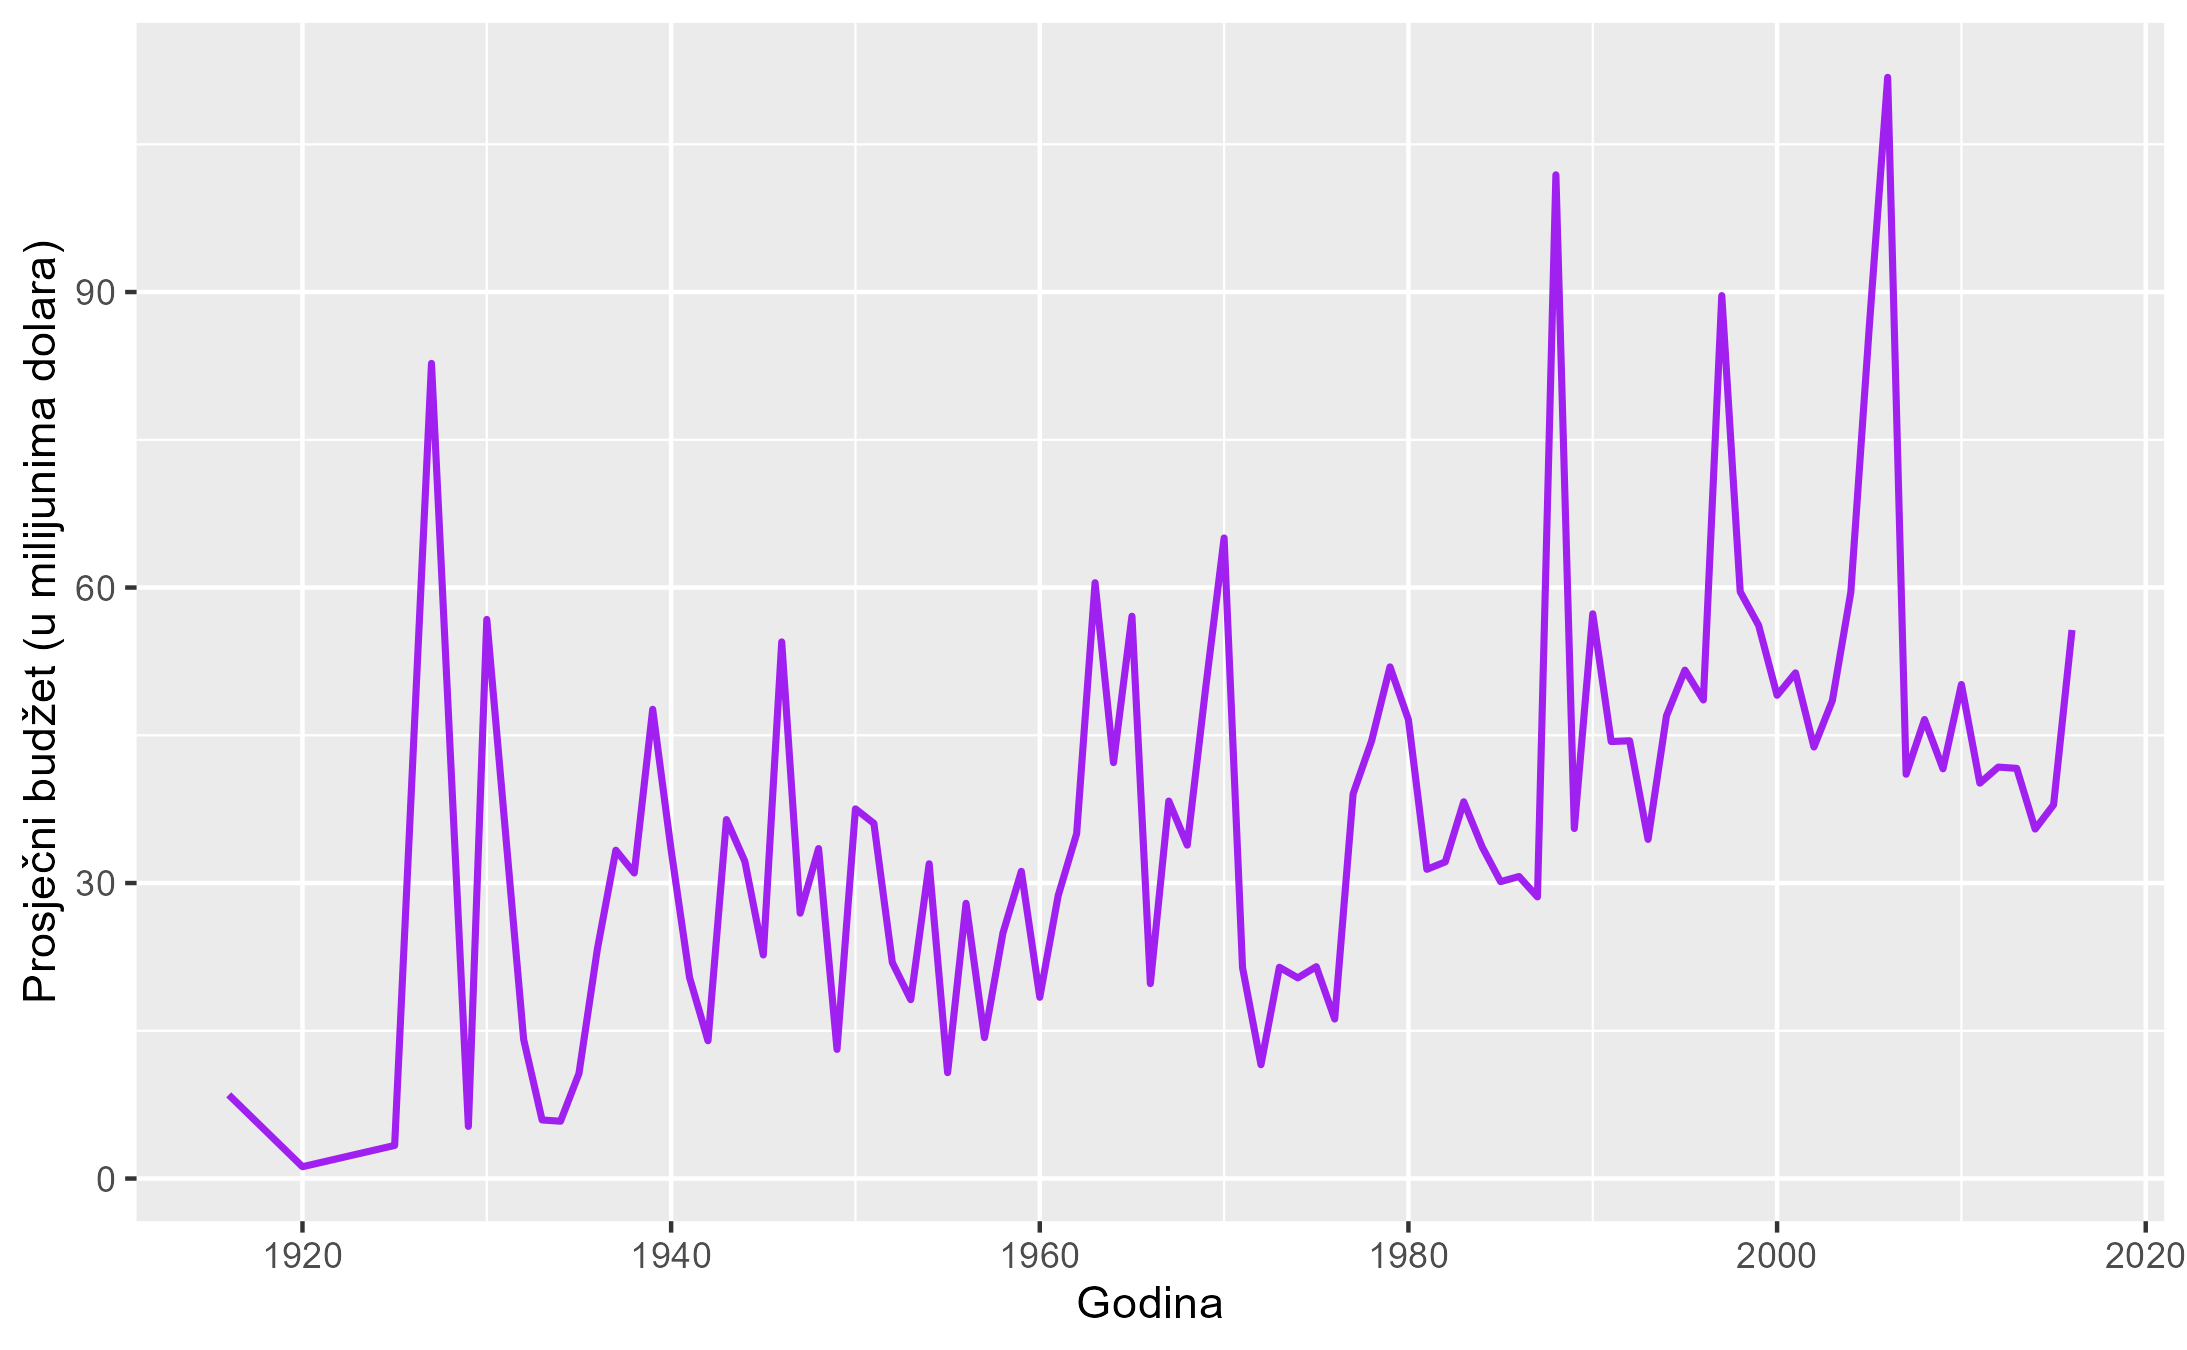
\includegraphics[width=15cm]{../figures/analysis/prosjecni_budzet.png}
		\caption{Prosječni budžet filmova po godinama}
		\label{budzet}
	\end{figure}
	
	
	
	
	
	
	
	
	
	
	